\chapter{Theoretical background}\label{theory}
In this section, I briefly introduce \gls{sota} methods and models used in the experiment section \ref{experiments}. Many of the problems in NLP are tasks of mapping one sequence to another; therefore, modern architectures were designed to tackle this very problem \textbf{efficiently}.




\section{Text representation}
In order to process text, NLP models operate on the text on a \textbf{token} level. A token can be understood as the smallest unit of text and is a product of a process called \textbf{tokenization} (transforming text into a set of tokens).

A typical token unit is a word; however, tokens can be as small as a single byte. Currently, a standard way of tokenization is using WordPiece tokens, which is a balance between word-level and byte-level tokenization.

After tokenization, a numerical representation of the tokens is to be obtained. A naive way is to use mapping for every word to an index in predefined/obtained vocabulary. Such approach suffers from the explicit ordering of the words, which may negatively influence the model. Another possible representation is \textbf{one-hot-encoding} where each word is represented by a vector that has $1$ in a single row and zeros everywhere else. The size of such an encoding is proportional to the size of the vocabulary, making the feature space very sparse. 

The current standard representations of words are word \textbf{embeddings}. Embeddings are fixed-size feature vectors. The dimension of the embeddings is a hyperparameter, usually with a value between 100 and 1000. Embeddings can be learned along the particular task, in an Embedding layer. Or, it is possible to use available precomputed representations, such as word2vec, Glove, or ELmo.
\newpage





\section{Neural Networks}
An \Gls{ann} is a model developed in the early 1940s \cite{mcculloch1943logical}. The smallest unit of a \Gls{nn} is a perceptron:
\begin{equation}
    f(x) = \phi(w^Tx + b)
\end{equation}
Where \textbf{weight} vector $w$ and \textbf{bias} term $b$ are learnable parameters, $x$ is an input feature vector and $\phi$ is an \textbf{activation function}. Activation functions are used for introducing non-linearities into the \Gls{nn}. In case of perceptron, it is a simple threshold function. Although the definition of \Gls{mlp} is loose, it can be understood as the simplest form of neural network with multiple connected perceptrons and a threshold activation function. In general, \Gls{nn}s usually use other activation functions such as sigmoid, ReLu, Tanh, LeakyReLu, etc.





\section{Encoder-Decoder}
Vanilla \Gls{nn} architecture operates on inputs of fixed length. For variable length input (for example, a sentence) \Gls{rnn} is used. Let $x = (x_1,x_2,...,x_T)$ be the input sequence. \gls{rnn} works on $x$ sequentially, updating its \textbf{hidden state} vector $h$ with some non-linear function, such as sigmoid, at each discrete time step. The final hidden state, also called \textbf{context vector} $c_T$, is preserved.
Therefore, \Gls{rnn} is able to map the input of arbitrary length $T$ to a fixed size vector $c_T$ that captures the information of the entire sequence.

The sequence-to-sequence \cite{sutskever2014sequence,cho2014learning} or \textbf{seq2seq} model aims to tackle the problem of mapping one sequence to another using two \Gls{rnn}s. The first \Gls{rnn} called \textbf{Encoder} is used to map the input sequence of arbitrary length to the fixed-size context vector. The context vector is then fed to a second \Gls{rnn} called \textbf{Decoder}. The decoder processes the context vector into a final sequence $y = (y_1,...,y_k)$, by updating its hidden state vectors while generating outputs $y_t$.

There are several problems with this architecture. Firstly, when a long sequence is processed, the information from earlier parts of the sequence is "forgotten". Secondly, RNNs work in a sequential manner; hence, there is no room for parallelism. The \textbf{Transformer} architecture aims to solve these problems.





\section{Transformers}\label{att_transformers}
Transformers is a family of deep neural architectures that has revolutionized the field of \gls{nlp}. The \textbf{attention} mechanism is a core principle behind transformer architecture and solves some of the problems mentioned in the previous section.

Current \gls{sota} language models, such as GPT-3, BERT, RoBERTa, all use the transformer architecture. Although their architecture can vary from the original one; for example BERT only uses the Encoder module. For the detection of \gls{mb}, I have eventually also narrowed the choice of models to transformers rather than other neural architectures.



\subsection{Attention}
Attention \cite{bahdanau2014neural,luongeffective} is essentially a mechanism that allows the unit (whether it is on the decoder or the encoder side) to learn to focus on some segments of the input sequence more than the others. This mechanism has been motivated by the problem of "forgetting" information in long sequences. This way, parts of the sequences that potentially drive the decision are represented more in hidden states than other less relevant parts.

\begin{figure}
  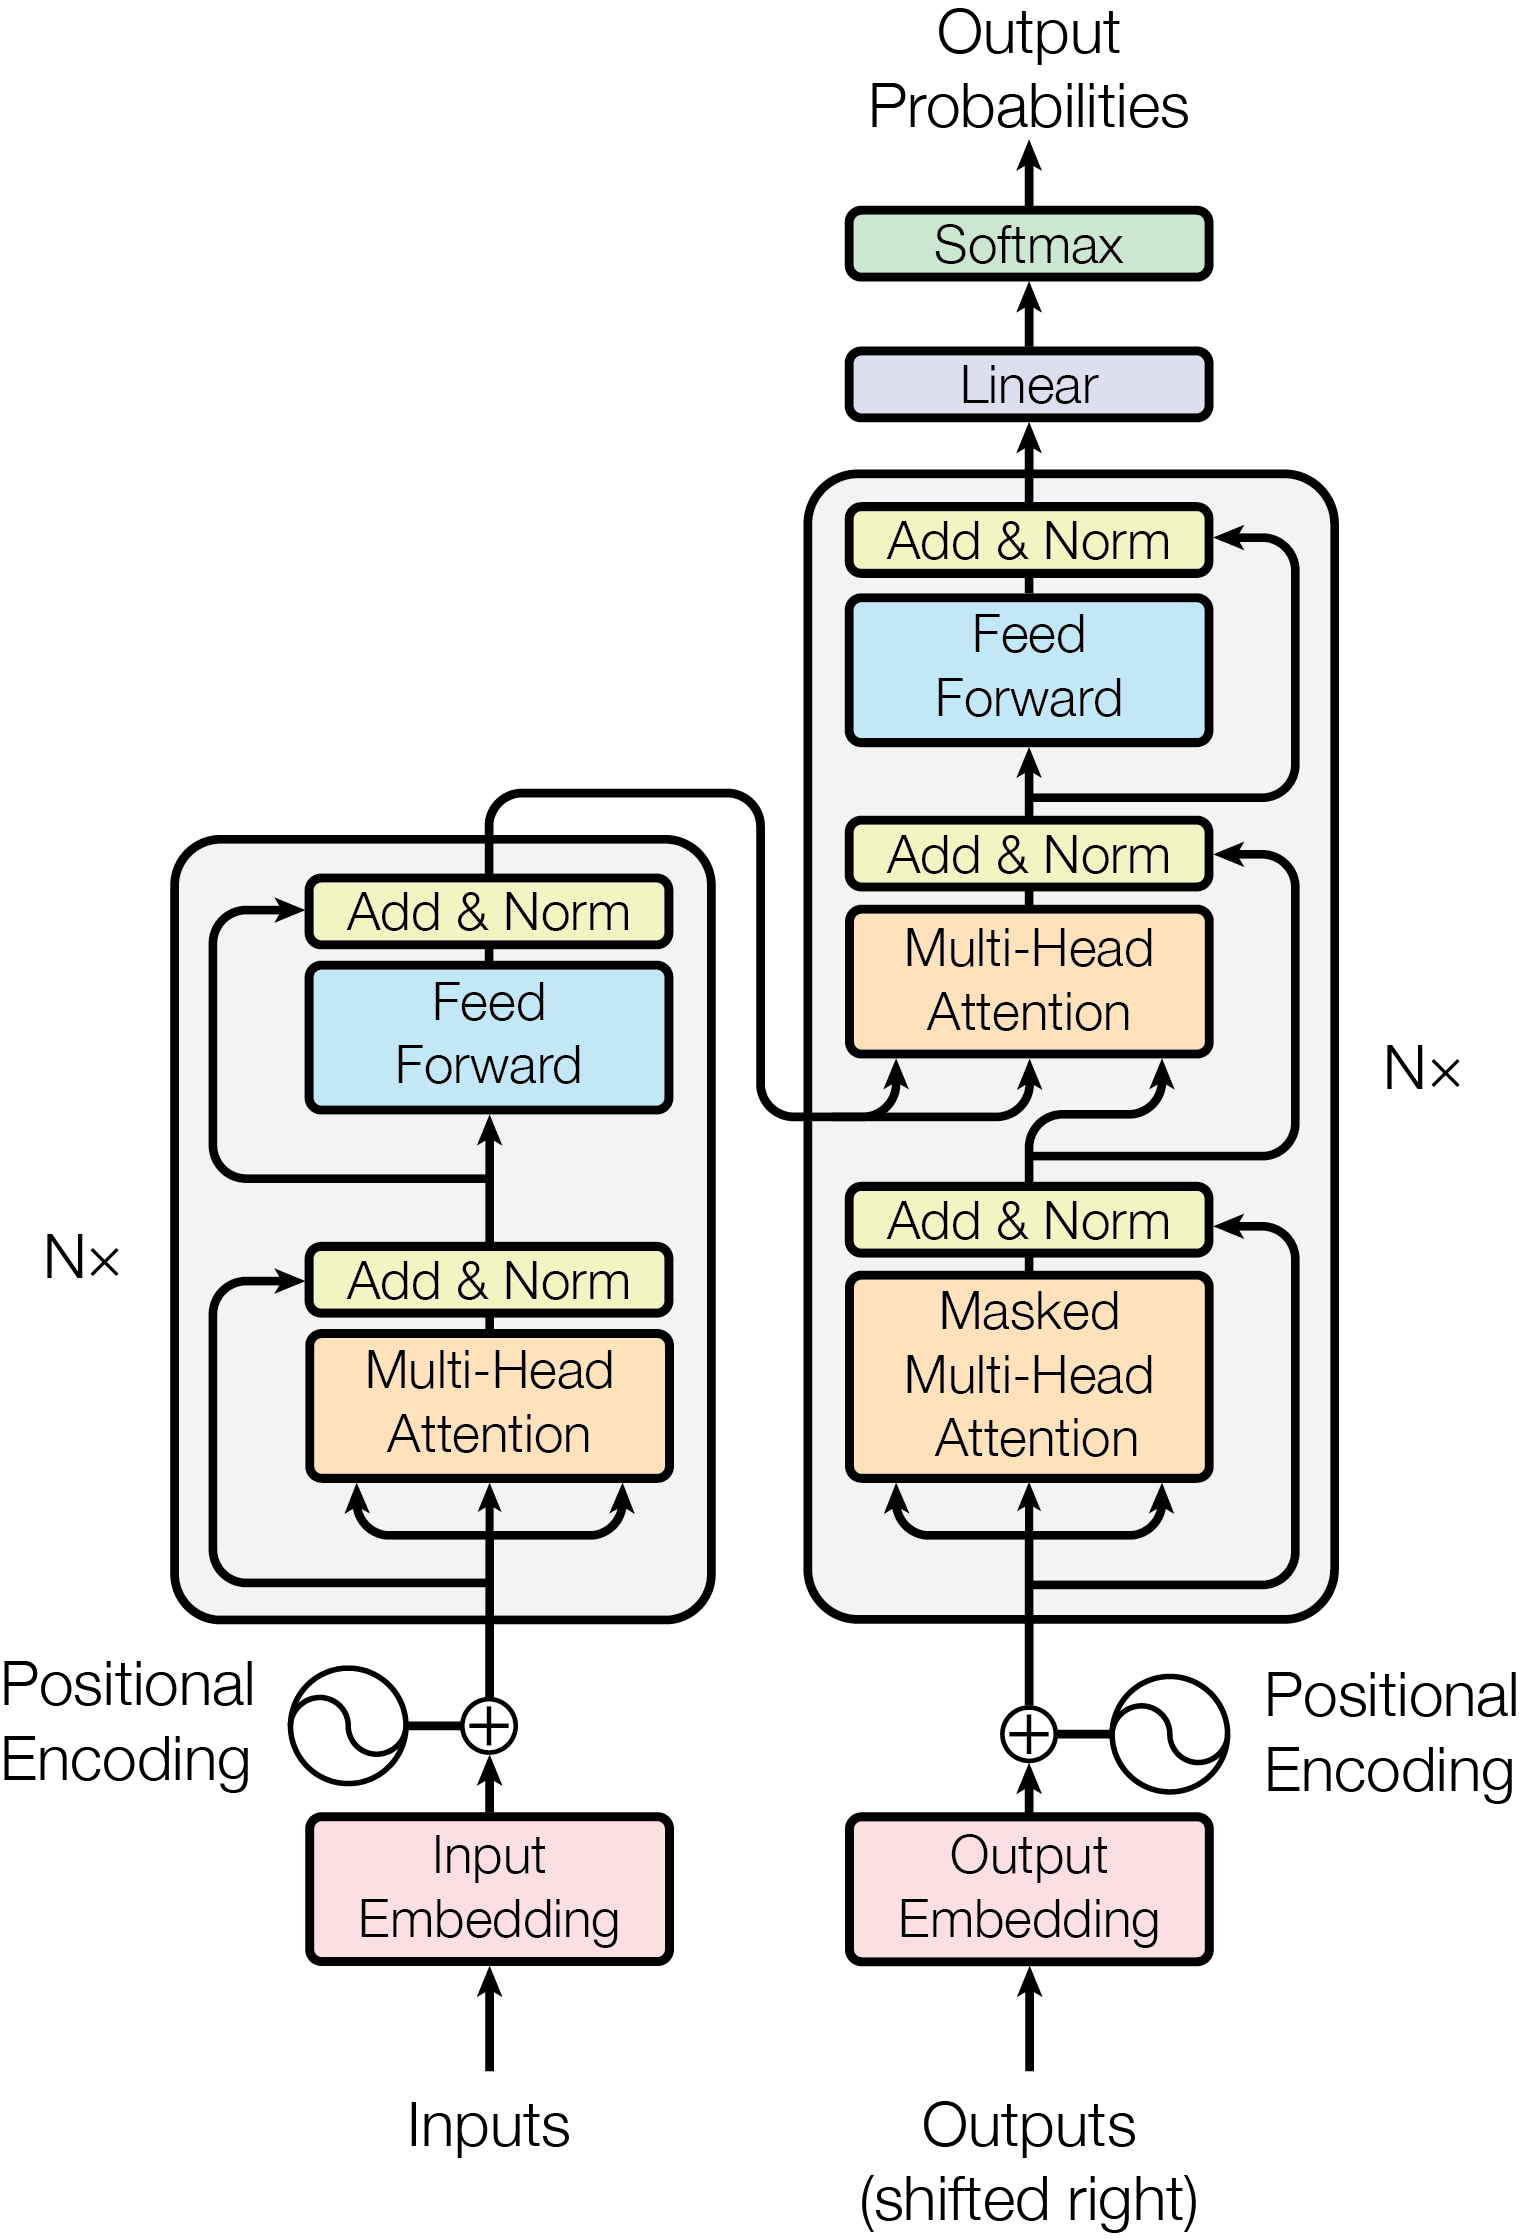
\includegraphics[scale=0.5]{my_modules/multimedia/atalyned.png}
  \caption{Transformer model architecture, preprinted reprinted from \cite{vaswani2017attention}}
  \label{fig:transformer}
\end{figure}

\subsection{Transformer architecture}
Scheme of the original architecture can be seen in \ref{fig:transformer}. The bottom of the architecture consists of an embedding layer enriched with \textbf{positional embeddings} that encodes the ordering information in the sequence.

Just as previous seq2seq models, the transformer also consists of Encoder and Decoder modules. Precisely, each module is a stack of $n$ identical encoder or decoder layers. Each encoder layer consists of two main layers: the \textbf{self-attention} layer and the \textbf{feed-forward} neural network.

As particular words/tokens flow through the stack of encoders, the model gradually builds up their representation. The self-attention layer uses the attention mechanism to incorporate other words from the sequence into each particular word representation. The original transformer architecture performs this self-attention computation eight times, allowing the model to learn different relationships between words. This is what the term \textbf{Multi-Head} attention refers to. The resulting representations from these heads are then concatenated and reduced in dimension to obtain the final representation to be fed to the feed-forward neural network. 

The Decoder modules work essentially the same, except it has an extra attentive layer that performs the attention computation over the output of the encoder stack. Since I only utilize the encoder part for more details, I refer the reader to the original transformer paper \cite{vaswani2017attention}.

Although the computation of self-attention is dependent on other tokens, the forward pass of a feed forward network can be done completely in parallel over the input sequence. Therefore, this design offers a significant computational speedup against the Encdoer-Decoder based on \gls{rnn}.




\section{Text classification}
Text classification is a supervised learning task of assigning a particular text (word, sentence, or document) a category to which it belongs. A standard loss for classification is a Cross-Entropy loss. In case of binary classification:

\begin{equation}
    L_{BCE} = \frac{1}{n} \sum_{i=1}^n ( y_i \cdot \log\hat{y_i} + (1-y_i)\cdot\log(1-\hat{y_i}))
\end{equation}

Where $y_i$ denotes the ground-truth label, $\hat{y_i}$ the probability predicted by the model, and $n$ is a number of samples.


    
\subsection{Metrics}
The most straight-forward way to evaluate the prediction ability of a classifier is to use the \textbf{accuracy} metric, which means counting correctly classified data. 
\begin{equation}
    accuracy = \frac{correct\ predictions}{total\ predictions}
\end{equation}
This metric is feasible if the classes of the dataset are balanced. However, imagine a situation where 90\% of the data belongs to one class and only 10\% to another. The classifier, which always outputs the first class, achieves 90\% accuracy even though its prediction capability is trivial. For unbalanced data, it is convenient to use the \textbf{F1} metric. The F1 score is a harmonic mean of \textit{Precision} and \textit{Recall}.

\begin{equation}
    F1 = \frac{2*Precision*Recall}{Precision + Recall}
\end{equation}
where precision

\begin{equation}\footnote{TP,TN,FP,FN denotes to True positive, True Negative, Fasle Positive, False Negative respectively.}
    Precision = \frac{TP}{TP+FP}
\end{equation}
can be understood as "how precisely the model predicts a positive class", whereas recall
\begin{equation}
    Recall = \frac{TP}{TP+FN}
\end{equation}
can be understood as "how much of a positive class can model predict".
The scores for each class are then averaged to obtain the final score. This is often referred to as "macro" averaging.




\subsection{Transformers for text classification}
The Predictive power of transformers is behind many \gls{sota} results, and text classification is no exception. For classification, usually only the encoder part of a transformer is utilized, although some define the classification problem as a sequence-to-sequence and incorporate the decoder too \cite{raffel2019exploring}.

During tokenization,a special [CLS] token is prepended to a sentence. The token has its own embedding and flows through the stack of encoders just as any other token, with a difference that when the forward pass reaches the classification layer, only the [CLS] token is passed as an input. [CLS] token can therefore be understood as a sort of sentence embedding.

Usually, one or two dense layers with an activation function are sufficient as a classifier on top of the encoder stack. However, it is also possible to extract representations from any level of the encoder stack and run an arbitrary classification algorithm on top of it.




\section{Transfer learning}
Nowadays, the true power of transformers lies in \textbf{transfer learning}. Transfer is a process where some knowledge is not learned from scratch but transferred from a previously trained model. Since large transformer models such as BERT or RoBERTa have millions of parameters, it would be extremely costly to train them from scratch. 

Such large models are usually pre-trained on an extensive corpus of data. There are several common \textbf{unsupervised} pre-training tasks that allow these models to learn contextual representations of words without supervision. For instance, \gls{mlm} is a task in which a random sample of tokens in the input sequence is replaced with a [MASK] token, and the model learns to predict the original token. Another unsupervised pre-training task is a \gls{nsp} which is self-explanatory.

Having such pre-trained model, one can then easily train a task specific head on top of pre-trained representations. Although the process of \textbf{fine-tuning} is more often adopted. During fine-tuning, the whole model with \textbf{all} its parameters is trained, as well as the task-specific head.

\section{Notes on Multi-Task learning}
When talking about training a neural network, we usually talk about fitting a network to one particular task. However, fine-tuning language models on small datasets often results in overfitting. Multi-Task learning \cite{caruana1997multitask} serves as a good \textbf{generalization} technique and a potential solution to this problem.

In essence, \gls{mtl} means learning multiple tasks together within one model; thus, representations for all tasks are learned together. Tasks do not have to share loss functions; they can have their own task-specific heads on top of the shared model.

In terms of optimizing (training) an \gls{mtl} model, there are two approaches in leveraging an \gls{mtl} paradigm \cite{ruder2017overview}.
\textbf{Hard-paramater sharing} where all parameters of the network, except the tasks-specific heads, are shared among tasks. On the other hand, with \textbf{Soft-parameter sharing}, each task has its own version of parameters, but they are encouraged to reduce the distance between the parameters through constraints.